\documentclass{article}

% if you need to pass options to natbib, use, e.g.: \PassOptionsToPackage{numbers, compress}{natbib}
% before loading nips_2016
% to avoid loading the natbib package, add option nonatbib: \usepackage[nonatbib]{nips_2016}

\PassOptionsToPackage{numbers, compress}{natbib}
\usepackage{nips_2016}
% to compile a camera-ready version, add the [final] option, e.g.:
%\usepackage[final]{nips_2016}

\usepackage[utf8]{inputenc} % allow utf-8 input
\usepackage[T1]{fontenc}    % use 8-bit T1 fonts
\usepackage{hyperref}       % hyperlinks
\usepackage{url}            % simple URL typesetting
\usepackage{booktabs}       % professional-quality tables
\usepackage{amsfonts}       % blackboard math symbols
\usepackage{nicefrac}       % compact symbols for 1/2, etc.
\usepackage{microtype}      % microtypography

\usepackage{amsmath,amsthm,color,graphicx,verbatim,listings,enumitem}
\graphicspath{{figures/}}

\lstset{
numbers=left, 
numberstyle=\small, 
numbersep=8pt, 
frame = single, 
language=matlab, 
framexleftmargin=20pt}

\newtheorem{lemma}{Lemma}

\title{A New Metropolis-Hastings Test for Fast Minibatch MCMC Inference and Optimization}

% The \author macro works with any number of authors. There are two commands used to separate the
% names and addresses of multiple authors: \And and \AND.
% Using \And between authors leaves it to LaTeX to determine where to break the lines. Using \AND
% forces a line break at that point. So, if LaTeX puts 3 of 4 authors names on the first line, and
% the last on the second line, try using \AND instead of \And before the third author name.

%%  David S.~Hippocampus\thanks{Use footnote for providing further
%%    information about author (webpage, alternative
%%    address)---\emph{not} for acknowledging funding agencies.} \\
%%  Department of Computer Science\\
%%  Cranberry-Lemon University\\
%%  Pittsburgh, PA 15213 \\
%%  \texttt{hippo@cs.cranberry-lemon.edu} \\


\author{
  John Canny \\
  Department of Computer Science \\
  University of California, Berkeley \\
  \texttt{canny@berkeley.edu}
  \And
  Haoyu Chen \\
  Department of Computer Science \\
  University of California, Berkeley \\
  \texttt{haoyuchen@berkeley.edu}
  \And
  Daniel Seita \\
  Department of Computer Science \\
  University of California, Berkeley \\
  \texttt{seita@berkeley.edu}
  \And
  Xinlei Pan \\
  Department of Bioengineering \\
  University of California, Berkeley \\
  \texttt{xinleipan@berkeley.edu}
  \And 
  Biye Jiang \\
  Department of Computer Science \\
  University of California, Berkeley \\
  \texttt{bjiang@berkeley.edu}
}

\begin{document}

\begin{comment}
\end{comment}

\maketitle

\begin{abstract}
Markov chain Monte Carlo (MCMC) methods are one of the most popular techniques in machine learning
for Bayesian inference. With large datasets, however, MCMC methods can be intractably slow due to
the need to compute the likelihood of all data points each iteration. Borrowing from the
optimization field, one way to make MCMC faster is to compute the posterior based on a random subset
of the data each iteration. Such stochastic MCMC has received increased research attention in recent
years, but these methods generally require adaptively increasing the minibatch size each iteration,
which can nullify the benefits if too much data is needed. In addition, with large datasets and
model optimization, it is unclear if obtaining a full posterior distribution is desirable over
getting a high-quality point MAP or ML estimate of the parameters.  In this paper, we present a new
Metropolis-Hastings test to fit in our alternative perspective on stochastic MCMC methods for big
data model optimization. We demonstrate the benefits of our approach with theoretical and empirical
results.
\end{abstract}



\section{Introduction}\label{sec:introduction}

Markov chain Monte Carlo (MCMC) sampling is one of the most popular techniques for Bayesian
computation. MCMC algorithms propose samples from a proposal distribution $q$, and decide whether to
accept or reject them based on a Metropolis-Hastings test~\cite{Metropolis1953,hastings70}. With
traditional Bayesian posterior inference, the posterior distribution $p(\theta \mid x_1, \ldots,
x_N) \propto p(\theta)\prod_{i=1}^np(x_i \mid \theta)$ of parameter $\theta$ based on conditionally
independent data $\{x_i\}_{i=1}^n$ is the target distribution which one aims to approximate by
sampling $\theta$ values. When $n$ is large (e.g., in the billions), it is computationally difficult
to compute the exact posterior because the likelihood must be evaluated on each $x_i$.

Recent success in machine learning optimization in the presence of large datasets have been in part
due to the ubiquitous use of stochastic gradient methods, where a subset of the data is used each
iteration to compute a noisy estimate of the gradient. These Robbins-Munro
algorithms~\cite{RobbinsMonro1951} have historically not been used with MCMC methods. A recent
result from~\cite{cutting_mh_2014} attempted to bridge the gap between minibatch optimization and
Bayesian inference by proposing an \emph{adaptive minibatch} method. Their method uses a subset of
the $N$ data points for the MH test each iteration, but requires incrementally increasing the
minibatch size so that it is more confident in its prediction on accepting or rejecting.

We argue for an alternative approach to using MCMC methods in the context of big data problems. In
general, model optimization involves finding one point estimate of optimal parameters based on a
user's goals, which typically refer to MAP or ML estimates. In addition, the more data one has, the
sharper the posterior distribution's modes. In the extreme case, the posterior would collapse to the
points corresponding to the modes, and it would be difficult for MCMC methods to escape.

Therefore, we are not interested in exact inference of the posterior model parameters for a very
large dataset, but rather, we want to perform either MAP or ML estimation. In both cases the goal is
to find a good posterior mode, but the exact form of the distribution is arbitrary. In particular,
non-unit powers of the distribution are fine. That corresponds to changing the temperature of the
distribution to make it ``flatter''.

Rather than fixing the posterior temperature and trying to use adjustable mini-batch size to achieve
it (which ends up reducing to nearly-full-batch updates) we propose to run at the natural
temperature induced by a given minibatch size. We can always increase the minibatch size to reduce
the temperature, but there is no need to do this beyond the point where the posterior mode is sharp
and well-defined. That will occur at some fixed number of points and far less than the full dataset.

To this end, we present a new Metropolis-Hastings test that can fit in this framework of minibatch
MCMC methods. We present theoretical and experimental results on our method and show that it can be
the method of choice for minibatch MCMC .




\section{Preliminaries and Related Work}\label{sec:related_work}

The standard MCMC method proceeds as follows~\cite{gilks1996markov,brooks2011handbook}. For a
parameter $\theta$ and conditionally independent data, we wish to compute the target distribution
$p(\theta \mid x_1, \ldots, x_N)$. Since exact evaluation is intractable, we generate a chain of
correlated samples $\theta_1, \ldots, \theta_T$ for some large $T$, and approximate $p$ by using
counts of samples. For each iteration $t$, we start with our current $\theta_t$. We use a
\emph{proposal distribution} $q(\theta' \mid \theta_t)$ to determine a new candidate $\theta'$. With
probability $P_a$, we accept it and set $\theta_{t+1} = \theta'$; otherwise, we repeat the previous
value $\theta_{t+1} = \theta_t$. Traditionally, $P_a$ is computed as follows:
\begin{equation}\label{eq:traditional}
P_a = \min\left\{ 1, \frac{f(\theta')q(\theta_t \mid \theta')}{f(\theta_t)q(\theta' \mid \theta_t)}
\right\} = \min\left\{ 1, \frac{p(\theta')\prod_{i=1}^N p(x_i ; \theta')q(\theta_t \mid \theta')}{p(\theta_t)\prod_{i=1}^N p(x_i ; \theta_t)q(\theta' \mid
\theta_t)} \right\},
\end{equation}
where $f(\theta_t)=p(\theta_t|x_1,\ldots,x_N) \propto p(\theta_t)\prod_{i=1}^N p(x_i \mid
\theta_t)$. The technical requirement for $P_a$ is that $f$ be proportional to the true target
distribution.

One then draws a uniform random variable $u$ from ${\rm Unif}[0,1]$ and accepts $\theta_{t+1} =
\theta'$ if $u < P_a$, and uses $\theta_{t+1} = \theta_t$ otherwise. The $P_a$ from
Equation~\ref{eq:traditional} satisfies detailed balance, so if one samples long enough using the
heuristic above, one will arrive at a stationary distribution.  The $P_a$ is guaranteed to converge
to the true $p$ distribution given sufficiently many examples (though a burn-in period and/or taking
every $n$th sample may be necessary).

Unfortunately, computing $f$ requires the use of all $N$ training data points. Moreover, it is
difficult to design tests using substantially fewer than $N$ points that also satisfy detailed
balance. There has been research on ways to conduct exact accept/reject tests using unbiased
estimators of the likelihood~\cite{Andrieu09thepseudo-marginal}. However, unbiased estimators of the
likelihood that can be computed from minibatches of data, such as the Kennedy-Bhanot
estimator~\cite{PhysRevD} have very high variance for large datasets. Because of this, once we get a
very high estimate of the likelihood, almost all proposed moves are rejected and the algorithm gets
stuck.

{\color{blue}
Daniel: I am worried. We need to motivate why it is not easy to use minibatch MCMC, and what other
researchers have tried to do about that.  The last paragraph is from~\cite{cutting_mh_2014}, and it
seems to argue that people have not used minibatch MCMC before ``the algorithm gets stuck''. But
isn't that exactly what our algorithm is doing when it is getting ``stuck'' at modes? If we wanted
to get stuck at modes with large datasets, why didn't we just do what previous work did?
}

The work of~\cite{cutting_mh_2014} proposes an adaptive minibatch approach by using a sequential
hypothesis testing algorithm. During each iteration, they start with a small minibatch of data and
test the hypothesis that the sample $\theta'$ should be accepted or rejected based the likelihood
ratio. If the test cannot make a decision over a certain confidence threshold, then they increase
the minibatch size and test again. This process repeats until a decision.  The downside of this
algorithm is the need to keep incrementing the mini-batch size in one iteration; in the worst case,
all $N$ data points may be needed in a single iteration. A related approach
is~\cite{icml2014c1_bardenet14}, which has slightly more robust theoretical properties, but comes at
the cost of more computational time. The work of~\cite{conf/uai/MaclaurinA14} presents an
\emph{exact} approach, but has the sometimes unreasonable requirement of a lower bound on the
per-datum likelihood factors.

There is a separate line of work related to optimizing MCMC about simulating the physics of a
probability distribution. By viewing random variables as ``particles'' in a system, it is possible
to apply Hamiltonian Monte Carlo (HMC)~\cite{mcmc_hamiltonian_2010} methods which generate both high
quality and distant proposals, getting the best of both worlds. These require a full gradient
computation of the posterior, which means they also suffer from the problem of needing to know the
likelihood at each point. Stochastic versions of HMC~\cite{sghmc_2014,stochastic_thermostats_2014}
use a minibatch of data each iteration but require controlling the noise from sampling so the sample
sequence does not diverge. A similar approach is to use Langevin
Dynamics~\cite{langevin_2011,conf/icml/AhnBW12}, which does not use the momentum terms in HMC.

Ultimately, minibatch SGHMC and Langevin Dynamics is an orthogonal contribution to ours, two ways of
attempting to solve the same problem of MCMC methods with big datasets. We could augment their
methods with our MH test, to get the benefit of their high quality proposals. Note that while their
methods in theory do not need an MH test, in practice, they need one due to discretization of the
system. Furthermore, tests may also be needed for when the algorithms are run with a constant step
size.

%% Daniel: I don't know how to integrate this easily.
%% \cite{sgmcmc_2015} (NIPS 2015) might want to give this a mention, where it would fit in their
%% recipe.



\section{A New Metropolis-Hastings Test}\label{sec:our_algorithm}

\begin{figure}[t]
  \centering
  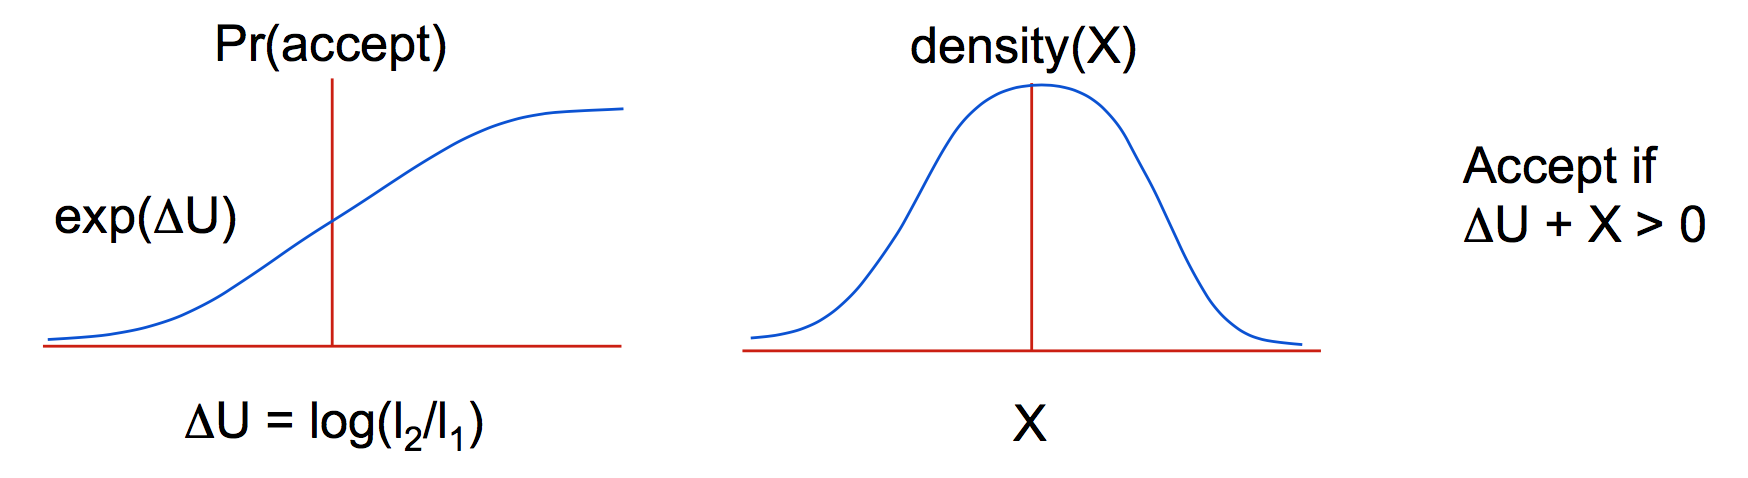
\includegraphics[width=\textwidth]{john_bair_fig01}
  \caption{
  To the left is the logistic distribution, representing a possible acceptance test. As $\Delta U$
  approaches infinity, the acceptance rate approaches 1. To the right, we have a new variable $X$
  and its density, along with an acceptance test $\Delta U + X$, which we describe in detail in
  Section~\ref{sec:our_algorithm} (note that we use $\Delta$ instead of $\Delta U$ for simplicity).
  {\color{blue}
  Daniel: I think that the diagram to the left should use the logistic function, i.e., replace
  ``$\exp(\Delta U)$'' with ``$(1+\exp(\Delta U))^{-1}$.''
  }
  }
  \label{fig:part1}
\end{figure}

\begin{figure}[t]
  \centering
  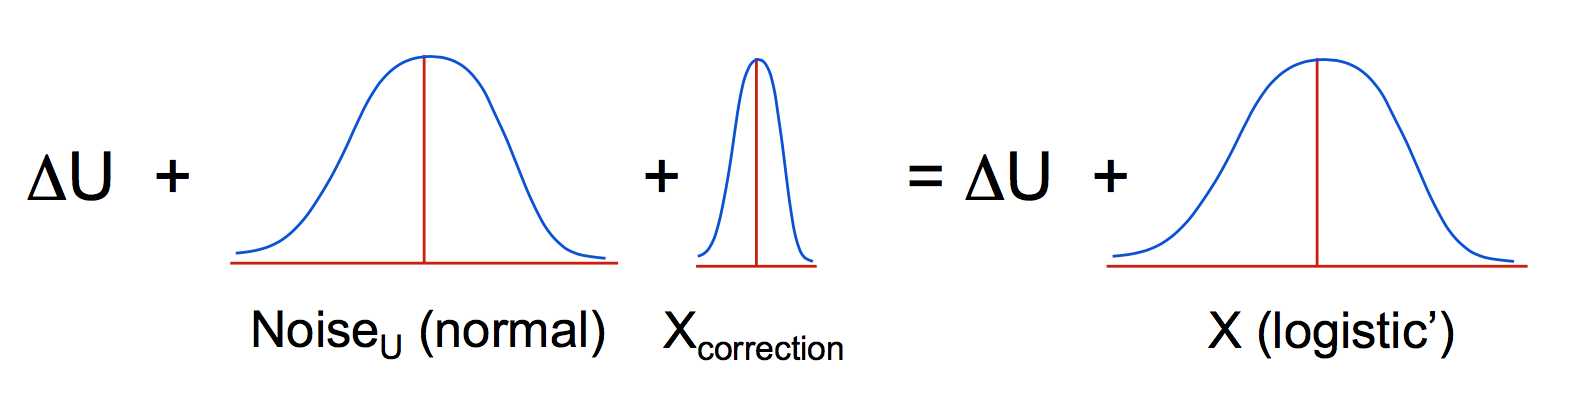
\includegraphics[width=\textwidth]{john_bair_fig02}
  \caption{
  To the left, we have $\Delta U$ (which is simplified as $\Delta$ in
  Section~\ref{sec:our_algorithm}), along with two noise terms that come from the new variable we
  define $X$. The details are in Section~\ref{sec:our_algorithm}.
  {\color{blue}
  Daniel: I think this needs to be merged into Figure~\ref{fig:part1}.
  }
  }
  \label{fig:part2}
\end{figure}

Our starting point is the following Lemma.

\begin{lemma}\label{lem:detailed_balance}
Let $\Delta = \log \left(\frac{f(\theta') q(\theta_t \mid \theta')}{f(\theta_t) q(\theta'\mid
\theta_t)} \right)$, where $f$ is proportional to the desired target distribution and $q$ is our
chosen proposal distribution. Any acceptance function $g$ such that $g(\Delta) = \exp(\Delta)
g(-\Delta )$ satisfies detailed balance. That is, $f(\theta_t)p(\theta' \mid \theta_t) =
f(\theta')p(\theta_t \mid \theta')$, where $p(\theta_y \mid \theta_x)$ is the probability of jumping
from $\theta_x$ to $\theta_y$ in our chain.
\end{lemma}

\begin{proof}
We begin by deriving $p(\theta' \mid \theta_t)$. This is equivalent to the probability of proposing
$\theta'$ and then accepting it, so
\begin{equation}\label{eq:one_way}
p(\theta' \mid \theta_t) = q(\theta' \mid \theta_t)g(\Delta).
\end{equation}
Similarly, we have
\begin{equation}\label{eq:other_way}
p(\theta_t \mid \theta') = q(\theta_t \mid \theta')g(-\Delta).
\end{equation}
Notice that the probability of accepting a transition from $\theta'$ to $\theta_t$ is $g(-\Delta)$
because this inverts the fraction inside the logarithm term of $\Delta$.  By assumption, we can
expand $g(\Delta) = \exp(\Delta)g(-\Delta)$ in Equation~\ref{eq:one_way}.  Doing this, and combining
the result of Equation~\ref{eq:other_way}, we get
\begin{equation}\label{eq:combined}
g(-\Delta) = \frac{p(\theta' \mid \theta_t)}{q(\theta' \mid \theta_t)\exp(\Delta)} = \frac{p(\theta_t \mid \theta')}{q(\theta_t \mid \theta')}.
\end{equation}
Rearranging terms and expanding $\exp(\Delta)$, we have
\begin{equation}\label{eq:rearrange}
\frac{p(\theta' \mid \theta_t) f(\theta_t) q(\theta' \mid \theta_t)}{q(\theta' \mid \theta_t) f(\theta') q(\theta_t \mid \theta')} = \frac{p(\theta_t \mid \theta')}{ q(\theta_t \mid \theta')}.
\end{equation}
Cancellations result in $f(\theta') p(\theta_t \mid \theta') = f(\theta_t) p(\theta' \mid \theta_t)$. Thus, detailed balance is satisfied.\\
\end{proof}

Some straightforward arithmetic shows that the standard Metropolis-Hastings acceptance function
$g(\Delta) = \min\{1, e^\Delta \} = \min\left\{1, \frac{f(\theta')q(\theta_t \mid \theta')}{f(\theta_t)q(\theta' \mid
\theta_t)}\right\}$ satisfies the condition $g(\Delta) =
\exp(\Delta)g(-\Delta)$ and consequently, results in detailed balance.

For reasons that will be clear later, we choose an alternative $g$, the logistic function:
$g(\Delta) = (1+\exp(-\Delta))^{-1}$. Again, straightforward arithmetic shows that it satisfies the
condition in Lemma~\ref{lem:detailed_balance}.

We can sample from the logistic function using the following procedure. Let $u$ be drawn from ${\rm
Unif}[0,1]$. At any given iteration, we can compute $\Delta$, and we accept the new candidate
$\theta'$ if $g(\Delta) > u$, and reject otherwise. Let us define the random variable $X =
g^{-1}(u)$ where again, $g$ is the logistic function. We claim that $X$ has CDF function $F_X(x) =
g(x)$, i.e., its CDF is precisely the logistic function. This is because for some $X = x$, we have
\[
F_X(x) = {\rm Pr}(X \le x) = {\rm Pr}(g^{-1}(u) \le x) = {\rm Pr}(u \le g(x)) = \int_{0}^{g(x)} 1 dx = g(x),
\]
as the density of the uniform random variable here is simply one. Thus, the criteria to accept the
candidate $\theta'$ is equivalent to whether $\Delta > X$, where $X$ has CDF of logistic function.
(If this isn't immediately obvious, note that we can pre-multiply $g^{-1}$ to $g(\Delta) \ge u$, and
our test is $\Delta > X$.) Since $X$ is symmetric about zero, the acceptance criteria can also be
expressed as $\Delta + X>0$, as shown in Figure~\ref{fig:part1}.

{\color{blue}
Daniel: The above makes sense, but I still don't understand why we had to show that the CDF of $X$
is the logistic function, because I never use that when I claim that our acceptance test is now
$\Delta > X$.  Do we need that assumption so that, for instance, we can decompose $X$ later the way
we do it, with $X_{\rm noise}$ having the same variance as $\epsilon$? That might explain it.
}

Unfortunately, there's a problem with the $\Delta + X > 0$ test: it requires us to compute $\Delta$,
so our test will be slow! We can get around this by defining a new scalar-valued term, $\Delta'$, which is
computed the same way as $\Delta$, but uses far fewer samples. In other words, $\Delta'$ is computed
based on a \emph{mini-batch} of data, and it is an approximation of $\Delta$, so we can express the
relationship as $\Delta' = \Delta + \epsilon$ for a noise term $\epsilon$. \emph{The key is that
$\epsilon$ follows a normal distribution}, $\epsilon \sim \mathcal{N}(0, \sigma^2)$, because for i.i.d. data $x_1, \ldots, x_N$, the $\Delta$
is expressed as the sum of log probabilities (look at Equation~\ref{eq:traditional} and apply the
logarithm to the product over the $N$ data points, to get a sum of log terms). All we do with
$\Delta$ is take far fewer of the summations, and normally-distributed noise is there as a product
of the Central Limit Theorem.

To sample accurately from $\Delta'$, we need to slightly change our acceptance criteria. We can
decompose $X$ as $X = X_{\rm norm} +X_{\rm correction}$, where the first term is a ``noise term''
which has the same variance as $\epsilon$, and the second term is a ``residual'' term. The criteria
to accept, previously expressed as $\Delta + X > 0$, can be rewritten as
\begin{equation}\label{eq:criteria}
\Delta + X = \Delta + X_{\rm norm} + X_{\rm correction} \approx \Delta' + X_{\rm correction} >0.
\end{equation}
This explains Figure~\ref{fig:part2} (though it really should be an approximation as we can't guarantee that our $X_{\rm norm}$ term is exactly the correct amount of noise), where the left hand side has distributions representing normal
noise ($X_{\rm norm}$, which is labeled as ${\rm Noise}_U$, but they are the same thing) and a
``correction'' term labeled $X_{\rm correction}$. Be aware that all of these ``additions'' are to be
interpreted as convolutions when computing the sum of densities.

Notice that we have several options we can control. For instance, we can adjust the mini-batch size;
increasing the mini-batch size will cause the $X_{\rm noise}$ distribution to shrink and become
narrower.

{\color{blue} Daniel: I think it's becoming clear but I'm still trying to connect all of the steps.
During each iteration of MCMC, we compute $\Delta'$ and \emph{sample} (right?) an $X$ (which we can
do by sampling $u$ and then doing $X = g^{-1}(u)$. This gives us $\Delta' + X$ but our MH test
    actually requires $X_{\rm correction}$, so first we must estimate $\sigma^2$, the variance of
    $X_{\rm noise} \sim \mathcal{N}(0, \sigma^2)$ (perhaps from the mini-batch data, somehow?) and
    then somehow ``remove'' that component from $X$ to get $X_{\rm correction}$? Then we have our
    acceptance test. Is this right? Or, of course, we don't have to sample $X$ at all, but just
    figure out a way to sample $X_{\rm correction}$ directly.

I think we talked about estimating $\sigma^2$. The variance $\sigma^2$ that we're concerned about is
a scalar value based on the sum of log probabilities of different samples, so one way we could
estimate the variance is by taking all samples of a mini-batch and seeing how much those individual
$\log p(x_i \mid \theta)$ vary. Or we could look at $k$ mini-batches of data which will give us
$\Delta_1, \ldots, \Delta_k$ and compute the empirical $\sigma^2$ (of course that defeats the
purpose of using mini-batches).  }

{\color{blue} Xinlei: I agree with you that out MH test requires $X_{correction}$. My understanding
is that we can actually estimate $X$ from the whole data set, and the probability distribution of
$X_{norm}$ is what we proposed? So the determination of $X_{correction}$ is a deterministic
deconvolution problem.  }




\section{Theoretical Results}\label{sec:theory}

TODO insert Haoyu's proof.

We implement our system within the open-source BIDMach project~\cite{canny2013bidmach}. Note to
ourselves: do NOT modify the \texttt{Learner.scala} code -- just make it a new ``Model''.




\section{Experiments}\label{sec:experiments}

\subsection{Mixture of Gaussians}\label{ssec:gaussians}

We start with a simple mixture of Gaussians.

\begin{figure}[ht]
  \centering
  \fbox{\rule[-.5cm]{0cm}{4cm} \rule[-.5cm]{4cm}{0cm}}
  %
\includegraphics[width=0.5\linewidth]{empty}
  \caption{This will be a sequence of images for the Gaussian mixture.}
\end{figure}

{\color{blue}
Daniel: TODO
}

\subsection{Logistic Regression}\label{ssec:logistic}

\begin{figure}[ht]
  \centering
  \fbox{\rule[-.5cm]{0cm}{4cm} \rule[-.5cm]{4cm}{0cm}}
  %
\includegraphics[width=0.5\linewidth]{empty}
  \caption{This will be a sequence of images for logistic regression.}
\end{figure}

{\color{blue}
Daniel: TODO
}

\subsection{Neural Network Optimization}\label{ssec:nets}

\begin{figure}[ht]
  \centering
  \fbox{\rule[-.5cm]{0cm}{4cm} \rule[-.5cm]{4cm}{0cm}}
  %
\includegraphics[width=0.5\linewidth]{empty}
  \caption{This will hopefully show results for neural networks on BIDMach.}
\end{figure}

{\color{blue}
Daniel: TODO
}




\section{Conclusions}\label{sec:conclusion}

{\color{blue}
Daniel: TODO
}


\small
\bibliography{nips_2016}
\bibliographystyle{ieeetr}
\normalsize

\clearpage
\appendix

\begin{center}
{\Large Outline of Appendix}
\end{center}

In this appendix, we describe the following topics, with an emphasis on clarity and understanding:

\begin{itemize}[noitemsep]
    \item Detailed discussion of the experiment from Section~\ref{ssec:gaussians}.
    \item Detailed discussion of the experiment from Section~\ref{ssec:logistic}.
    \item Detailed discussion of the experiment from Section~\ref{ssec:nets}.
\end{itemize}

\section{Gaussian Mixture Experiment Details}

\subsection{Mathematical Assumptions}

We borrow this example from~\cite{langevin_2011}. Our parameter is a 2-D vector $\theta =
(\theta_1, \theta_2)$, where
\begin{equation}
\theta_1 \sim \mathcal{N}(0, \sigma_1^2) \quad \mbox{ and } \quad \theta_2 \sim \mathcal{N}(0, \sigma_2^2)
\end{equation}
where $\mathcal{N}$ indicates the normal distribution (more generally, the multivariate normal). We
consider the above as our prior. Following~\cite{langevin_2011}, we set $\sigma_1^2 = 10$ and
$\sigma_2^2=1$, so the covariance matrix of $\theta$ is $\Sigma = {\rm diag}(10,1)$. Therefore, the
log prior probability we endow on $\theta$ is
\begin{equation}
\log p(\theta) = \log \left(\frac{1}{2\pi\sqrt{10}}\right) - \frac{1}{2}\theta^T\Sigma^{-1}\theta.
\end{equation}
To generate the data, we use the following Gaussian mixture with tied means:
\begin{equation}\label{eq:x_points}
x_i \sim \frac{1}{2}\mathcal{N}(\theta_1, \sigma_x^2) + \frac{1}{2}\mathcal{N}(\theta_1+\theta_2, \sigma_x^2)
\end{equation}
where, again following~\cite{langevin_2011}, we set $\sigma_x^2 = 2$. This means the log likelihood
of a single data instance is
\begin{equation}
\log p(x_i \mid \theta) = \log\left(\frac{1}{4\sqrt{\pi}}\right) +
\log\left(\exp\left(-\frac{1}{4}(x_i - \theta_1)^2\right) + \exp\left(-\frac{1}{4}(x_i -
(\theta_1+\theta_2))^2\right)\right)
\end{equation}
Here is the problem statement. Given some number of i.i.d. data points $x_1, x_2, \ldots, x_N$
generated according to~(\ref{eq:x_points}), determine the posterior distribution\footnote{Note that,
as is typical with Bayesian analysis, we do not concern ourselves with the denominator of the
original (non-log) posterior.} of $\theta$:
\begin{equation}\label{eq:log_post}
\log p(\theta \mid x_1,\ldots,x_N) = \log p(\theta) + \sum_{i=1}^N\log p(x_i \mid \theta).
\end{equation}
Alternatively, if there are too many data points, we may opt to instead pick a point estimate of
$\theta$, generally the MAP estimate. (If $N$ is extremely large, it will cause the posterior to
peak sharply at its modes, reducing distribution estimates to point estimates.) Note that in many
cases, we will need to take a \emph{minibatch estimate} of~(\ref{eq:log_post}). In that case, the
literature generally uses
\begin{equation}\label{eq:scaling_factor}
\log p(\theta \mid x_1,\ldots,x_N) \approx \log p(\theta) + \frac{N}{n} \sum_{i=1}^n\log p(x_i \mid \theta).
\end{equation}
where we only use $n \ll N$ samples, but we must scale up the likelihood contribution by $N/n$. If we
didn't add this scaling factor, then the contribution of the likelihood terms would be weaker. There
is another thing we need to consider about that, which is the \emph{temperature} of our
distribution. In general, we will want to add $T > 1$ so that our posterior is
$p(\theta)((\prod_{i=1}^n p(x_i\mid \theta))^{N/n})^{1/T}$, resulting in the log
posterior of 
\begin{equation}\label{eq:log_prior_temp}
\log p(\theta \mid x_1,\ldots,x_N) \approx \log p(\theta) + \frac{1}{T}\frac{N}{n} \sum_{i=1}^n\log p(x_i \mid \theta).
\end{equation}
which has the extra $1/T$ to decrease the scale factor.  Equation~(\ref{eq:log_prior_temp}) is what
we will be using for our experiments, because we need to consider warmer distributions.
{\color{blue} Daniel: not totally confident on this but I'll try.}

Finally, recall earlier that we needed to define $\Delta$. In our context, $\Delta$ is:
\begin{align}
\Delta &= \log \left(\frac{f(\theta') q(\theta_t \mid \theta')}{f(\theta_t) q(\theta'\mid \theta_t)} \right) \\
&= \log p(\theta') - \log p(\theta_t) + \sum_{i=1}^N(\log p(x_i \mid \theta') - \log p(x_i \mid \theta_t)) + \log\left(\frac{q(\theta_t \mid \theta')}{q(\theta' \mid \theta_t)}\right).
\end{align}
But again, with \emph{minibatches} of data, we usually do not sum over all $N$ terms and instead sum
over $n$ terms, but with the extra $(1/T)(N/n)$ scaling factor, from
Equation~(\ref{eq:log_prior_temp}). We generally denote that approximation as $\Delta'$ in the paper.

\subsection{Experiment Observations}

\begin{figure}[t]
  \centering
  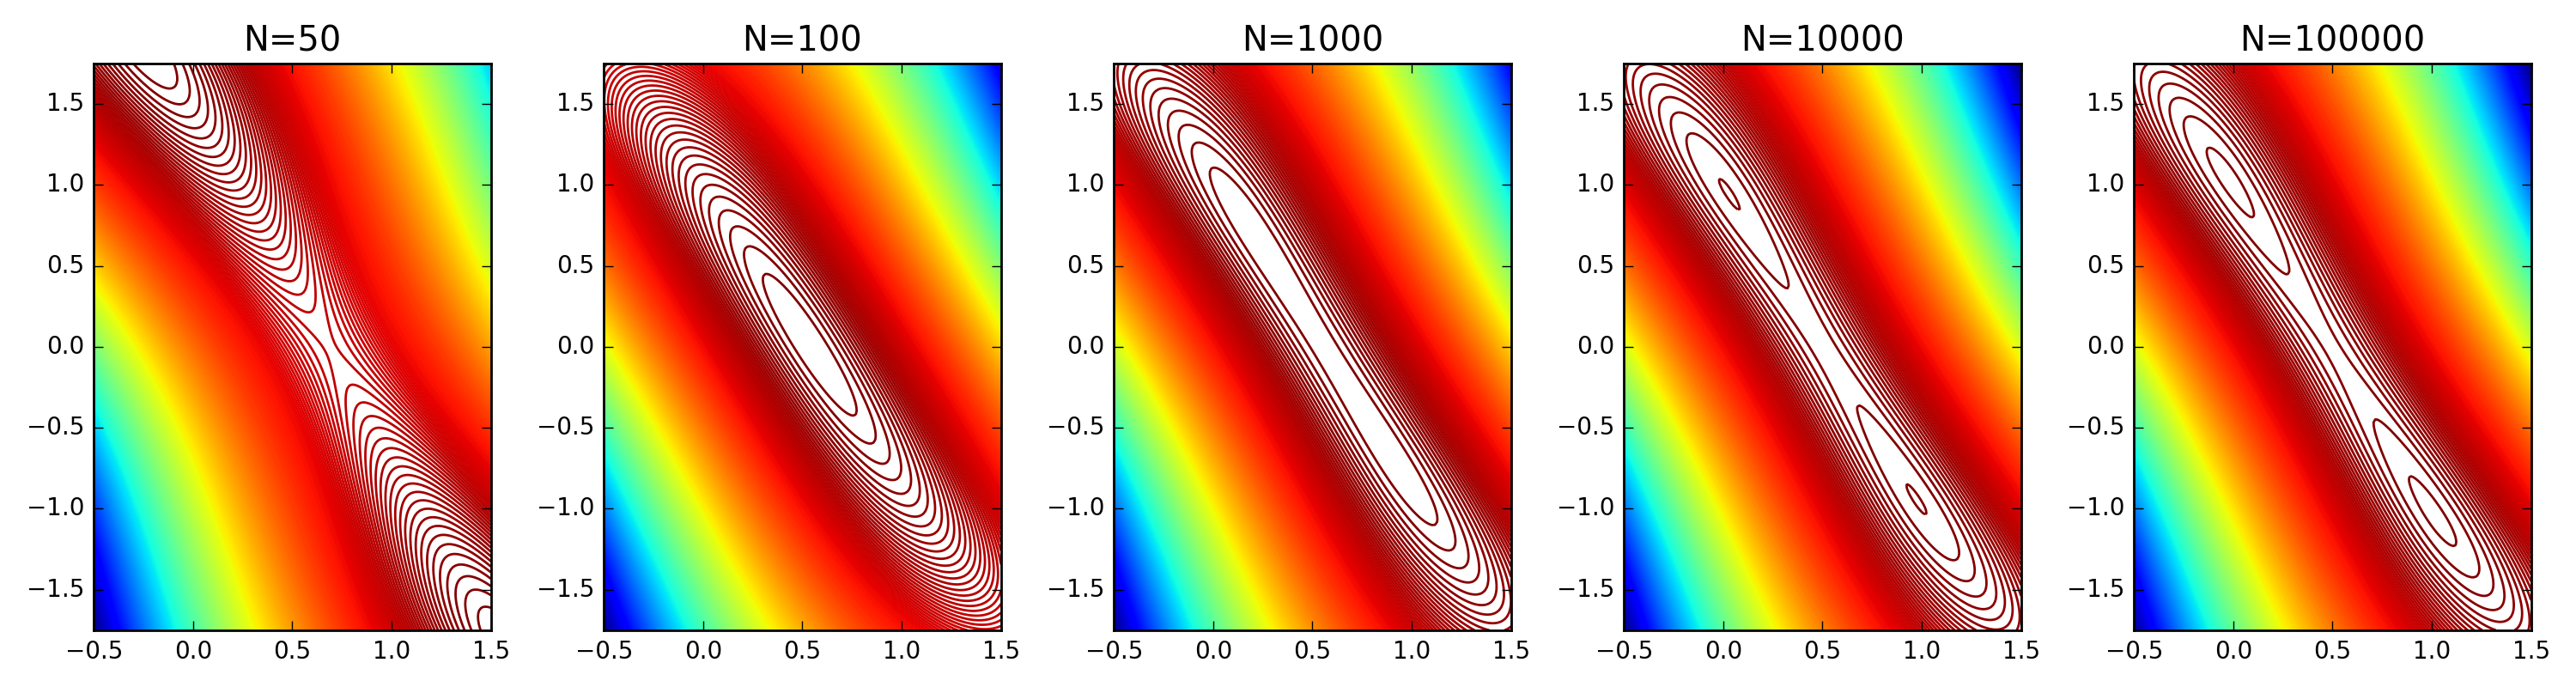
\includegraphics[width=1\linewidth]{contour_v1}
  \caption{The posterior distribution, from 50 to 100k samples, with temperature set at 1.}
  \label{fig:contour1}
\end{figure}
\begin{figure}[t]
  \centering
  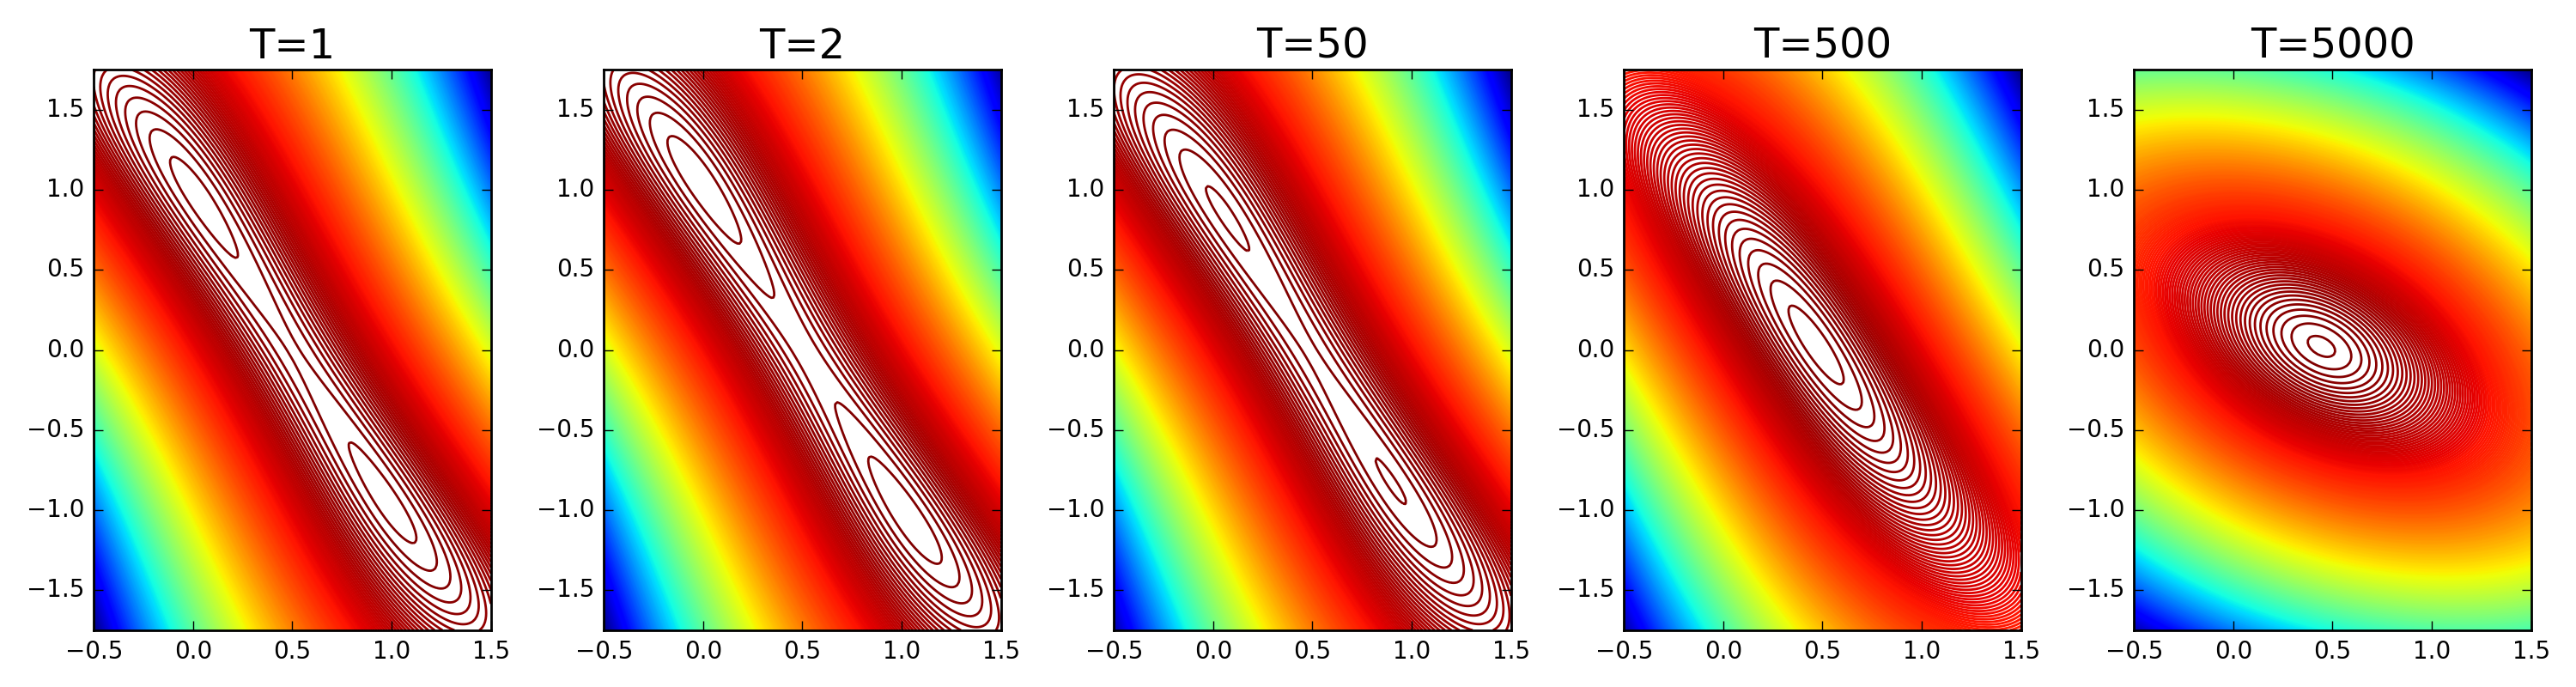
\includegraphics[width=1\linewidth]{contour_v2}
  \caption{The posterior distribution, with $N=10000$ but with temperature $T$ varying.}
  \label{fig:contour2}
\end{figure}

In this experiment, we compare our method with the one from~\cite{cutting_mh_2014}, hereafter called
the ``adaptive sampling approach''. We apply them to the Gaussian Mixture model previously
discussed.

Figure~\ref{fig:contour1} shows simulated contour plots of the posterior based on the $N$ data
points, for varying $N$, with the temperature set at $T=1$. Note that because we're using all $N$
points here, the scale factor $N/n=1$. As $N$ increases, the posterior converges to a multimodal
distribution with modes at $(0,1)$ and $(1,-1)$. 

Figure~\ref{fig:contour2} is similar, except this time we fix the number of samples at $N=10000$,
but show how changing the temperature $T$ affects the distribution. A larger $T$ implies a flatter
posterior, one that (weakly) peaks in between the two true modes.

Our ultimate goal is to either (a) get a posterior distribution that covers the posterior well, or
(b) to get samples that stay trapped at a mode, for a point estimate of $\theta$.  Whether our goal
is (a) or (b) depends on our objectives and the context of the problem (e.g., big data usually
implies (b) is OK even if it would not satisfy the average Bayesian).

For both our method and the adaptive sampling method, we use random walk proposals. (Thus, the term
in $\Delta$ containing the $q$s disappears.)  Random walk proposals are bad, but since the proposal
is poor, good performance can only be obtained with a strong MH test, hence why we can use this as a
reasonable starting benchmark.

We test use the following settings:

\begin{itemize}[noitemsep]
    \item We use $N=10000$ samples of $x_i$.
    \item The covariance of the Gaussian random walk is ${\rm diag}(0.1, 0.1)$.
    \item We use 10000 iterations. One iteration involves one $\theta'$ proposal and a test to
    accept/reject.
    \item The mini-batch size is set at 100, so it is one percent of the total data. For the
    adaptive sampling approach, this is the amount that the minibatch size would keep increasing if
    we needed more precision. Our approach, of courses, keeps the size fixed.
    \item For adaptive sampling, the tolerance for deciding on a test is 0.05. The temperature for
    that is also set at $T=1$ because that algorithm was not designed to deal with temperatures.
    \item For our approach, to get an estimate of the standard deviation of $\Delta'$ (remember,
    $\Delta'$ is a minibatch approximation of $\Delta$) we take five other minibatches (randomly
    selected from the data) and take the standard deviation of those values.
\end{itemize}

For our approach, we run using three different temperature values, $T=1$, $T=10$, and $T=100$.

Figure~\ref{fig:scatter} compares scatter plots of the ``Cutting the MH'' test (hereafter called
``adaptive minibatch'') versus ``Our Method'', where we use three different temperature settings.
There doesn't seem to be too much noticeable difference in our method for the three different
temperature setting values, but our approach is a lot different from the adaptive sampling method
(this is because of rejection rates, more on that later).

\begin{figure}[ht]
  \centering
  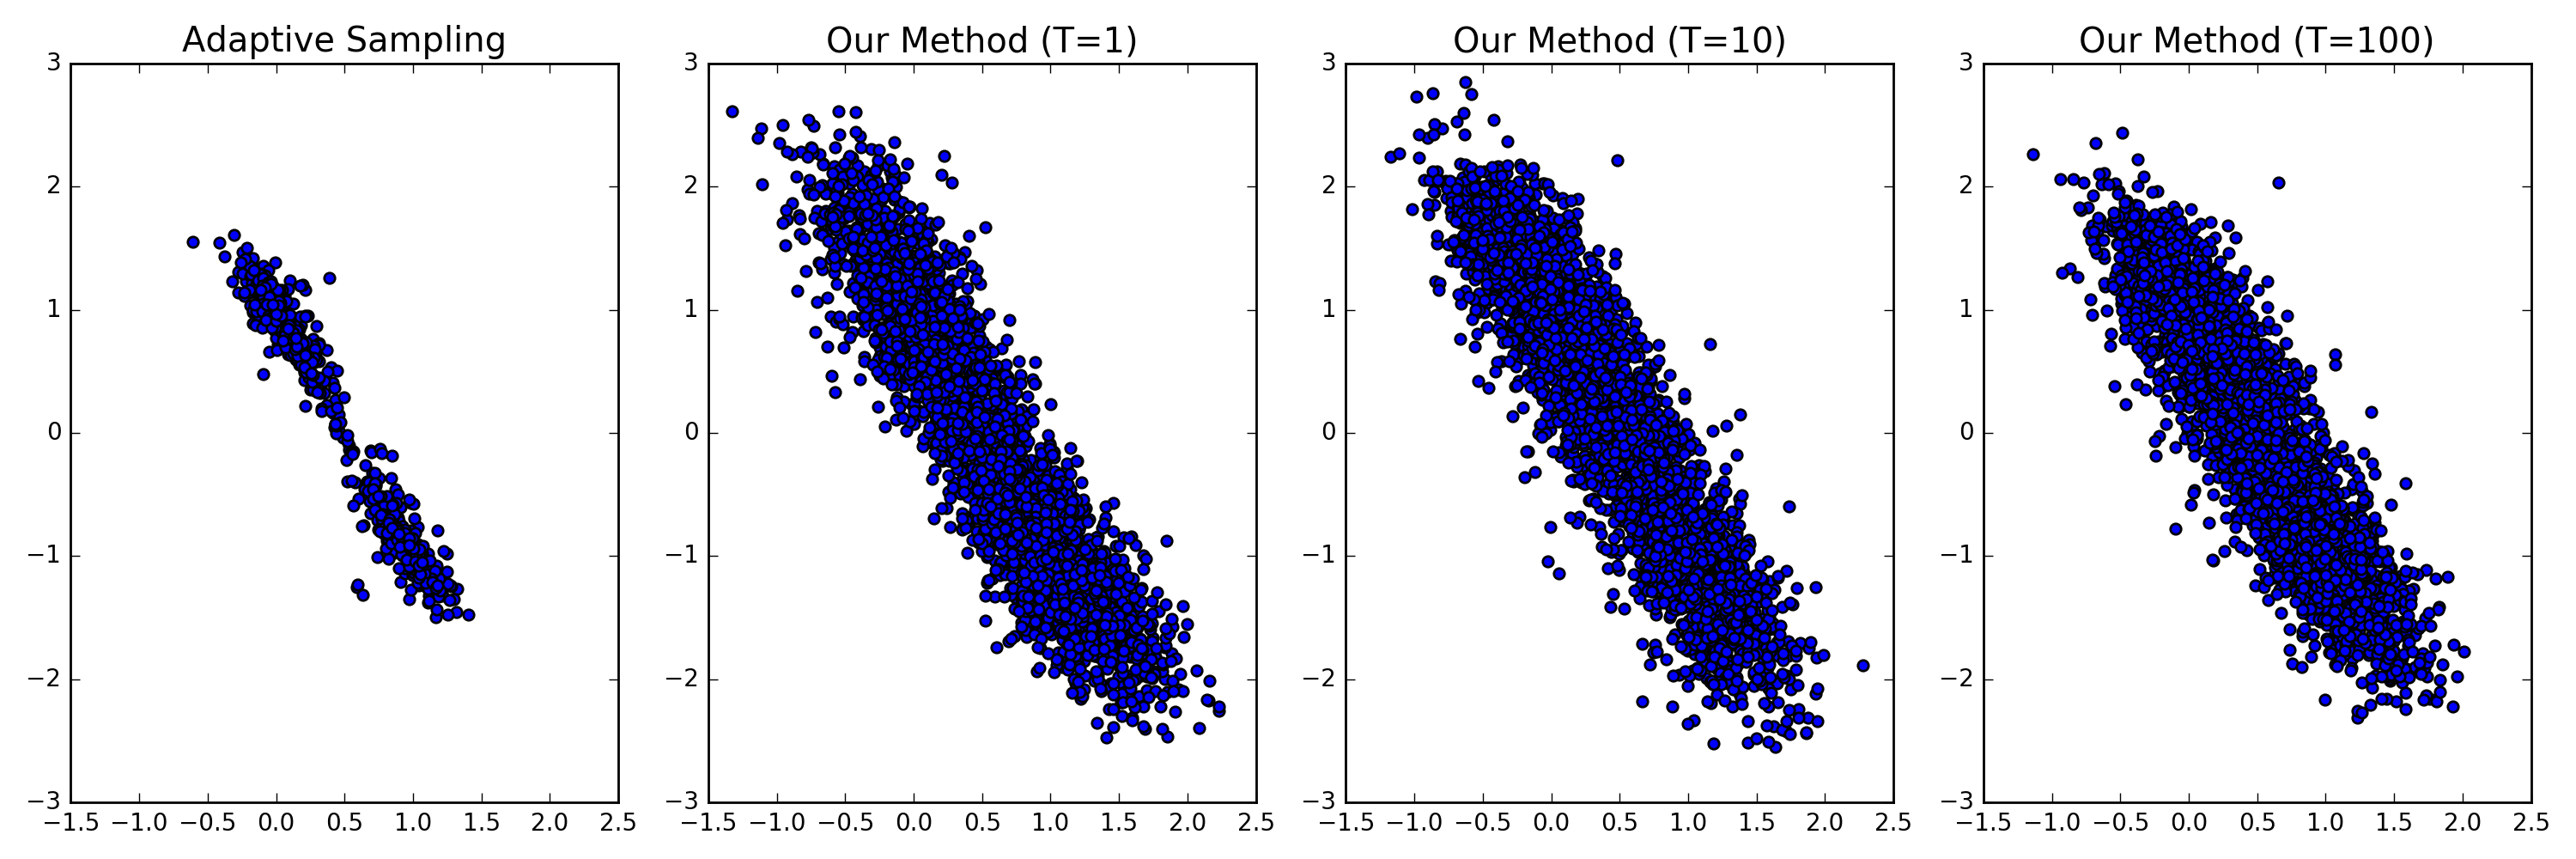
\includegraphics[width=1\linewidth]{scatter_v01}
  \caption{Scatter plots of accepted $\theta$ for (in order) the adaptive sampling approach, and our
  method (temperatures 1, 10, and 100).}
  \label{fig:scatter}
\end{figure}

Before taking a look at our approach, we first examine the adaptive sampling approach. \textbf{That
approach rejected a lot of samples; out of 10000 iterations, it only accepted 773 times}.
Figure~\ref{fig:mb_sizes} describes the histograms of the adaptive minibatch's batch sizes. (Note
that the histogram y-axis values are different.) In many cases, using the initial batch size of 100
sufficed to make an accept/reject decision, but sometimes, this method needed to use the entire 10k
data set. Decreasing the tolerance (from its current 0.05 value) would have required larger
minibatches. Incidentally, it makes sense that the method rejects a lot of samples, because the
random walk proposal usually provides us with poor points.

\begin{figure}[ht]
  \centering
  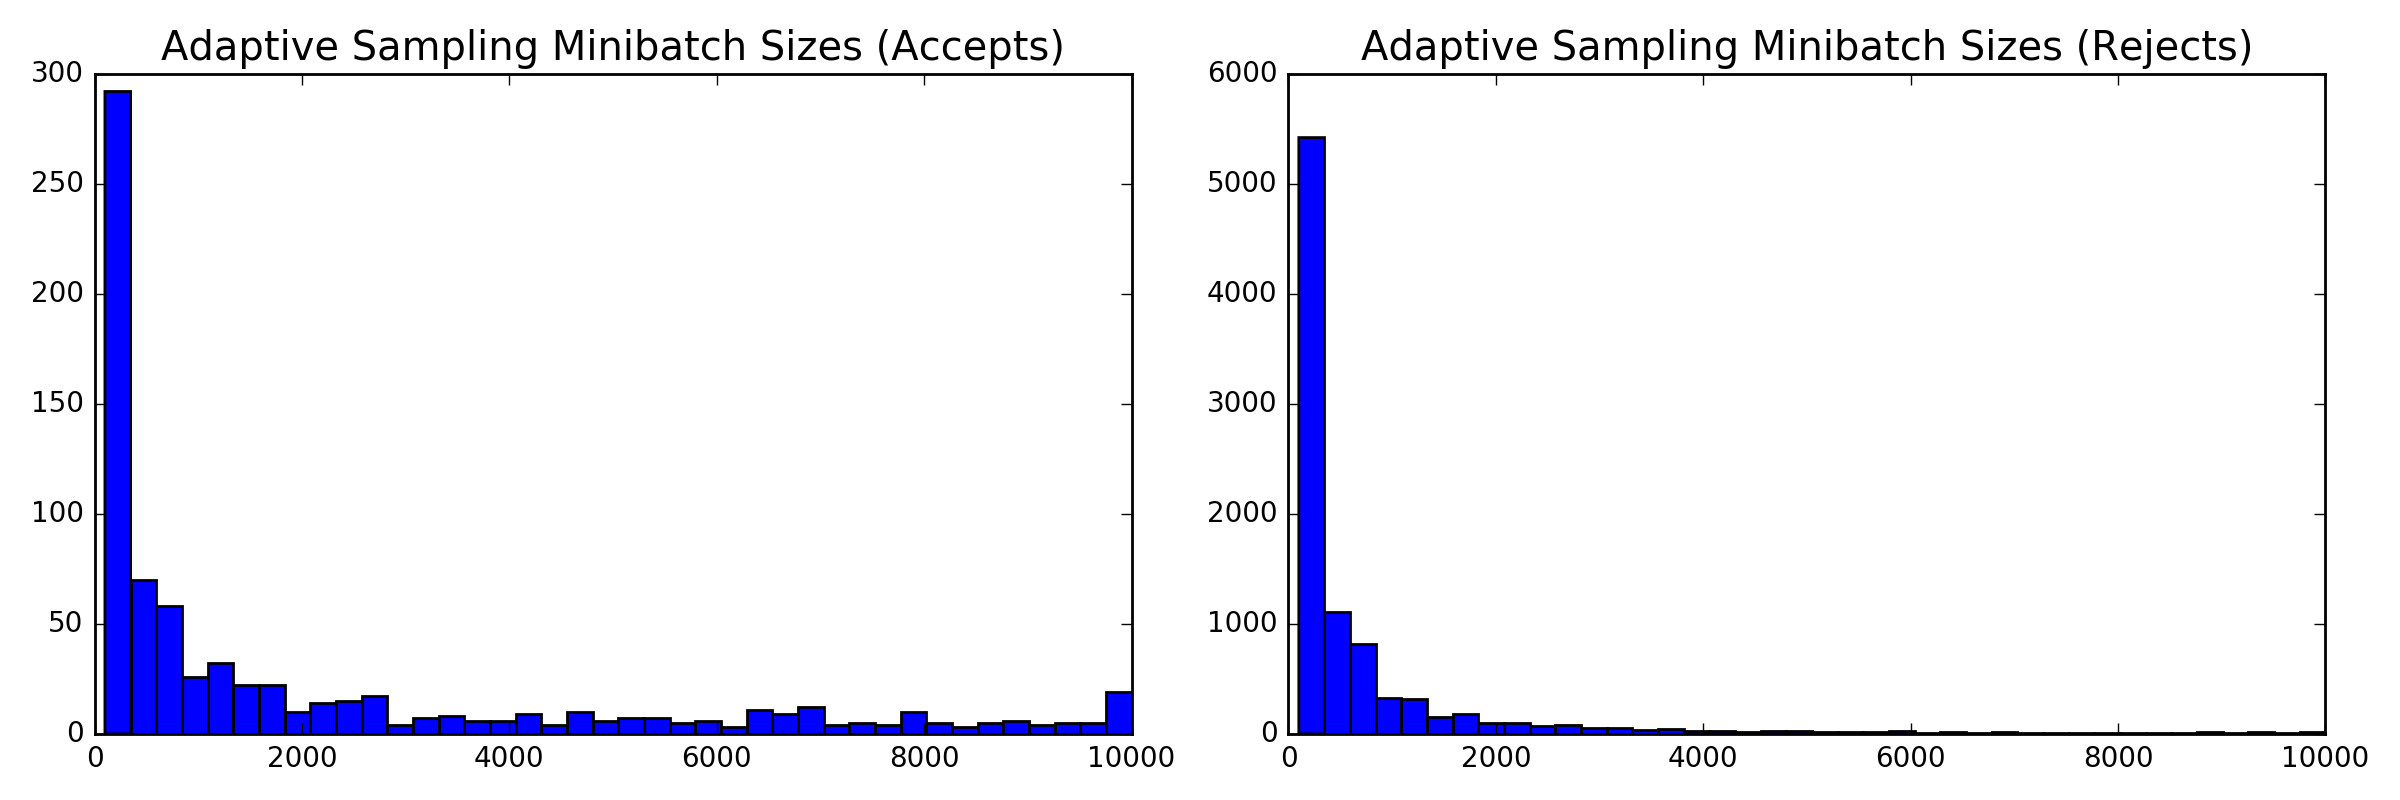
\includegraphics[width=0.75\linewidth]{adaptive_sampling_sizes_v01.png}
  \caption{Minibatch sizes for adaptive sampling when it was accepting or rejecting.}
  \label{fig:mb_sizes}
\end{figure}

Now we analyze our approach in more detail. Our method accepts far more samples than the adaptive
sampling method, \textbf{accepting 3285, 3318, and 3332 out of 10k}, for temperature values 1, 10,
and 100, respectively.

For diagnostics purposes, Figures~\ref{fig:diagnostics1},~\ref{fig:diagnostics2},
and~\ref{fig:diagnostics3} express histograms (for all three temperature runs) of the $\Delta'$,
${\rm std}(\Delta')$, and $X_{\rm corr}$ values, respectively.

There are a few immediate observations. First, increasing the temperature size by a factor of 10
will decrease $\Delta'$ by a factor of 10, which makes sense. That will also directly affect the
standard deviation estimate of $\Delta'$. Our $X_{\rm corr}$ distribution is symmetric about zero,
which is also expected (and it also exhibits a decrease in a factor of 10 for an increase
in temperature).

{\color{blue}
One concern I have is that our $\Delta'$ values do not seem to be ``sufficiently negative''. If our
$\Delta'$ values are negative (but large in absolute value) that means our MH test will reject more
often. But then this raises another concern: didn't we say at one point that we \emph{should} be
getting high acceptance rates, around 50 percent (in part because of the shape of the logistic
function)? Doesn't that depend on the quality of the proposal distribution? If our method is
designed to accept a lot regardless of the proposal distribution, I don't see how its performance
can be considered equal to the adaptive sampling approach, or even a standard MH test. In fact, the
best observation I can derive from this is that our approach and the adaptive sampling (or any
standard MH test) will accept the high likelihood cases, but our case will accept the borderline
ones more often.
}

\begin{figure}[ht]
  \centering
  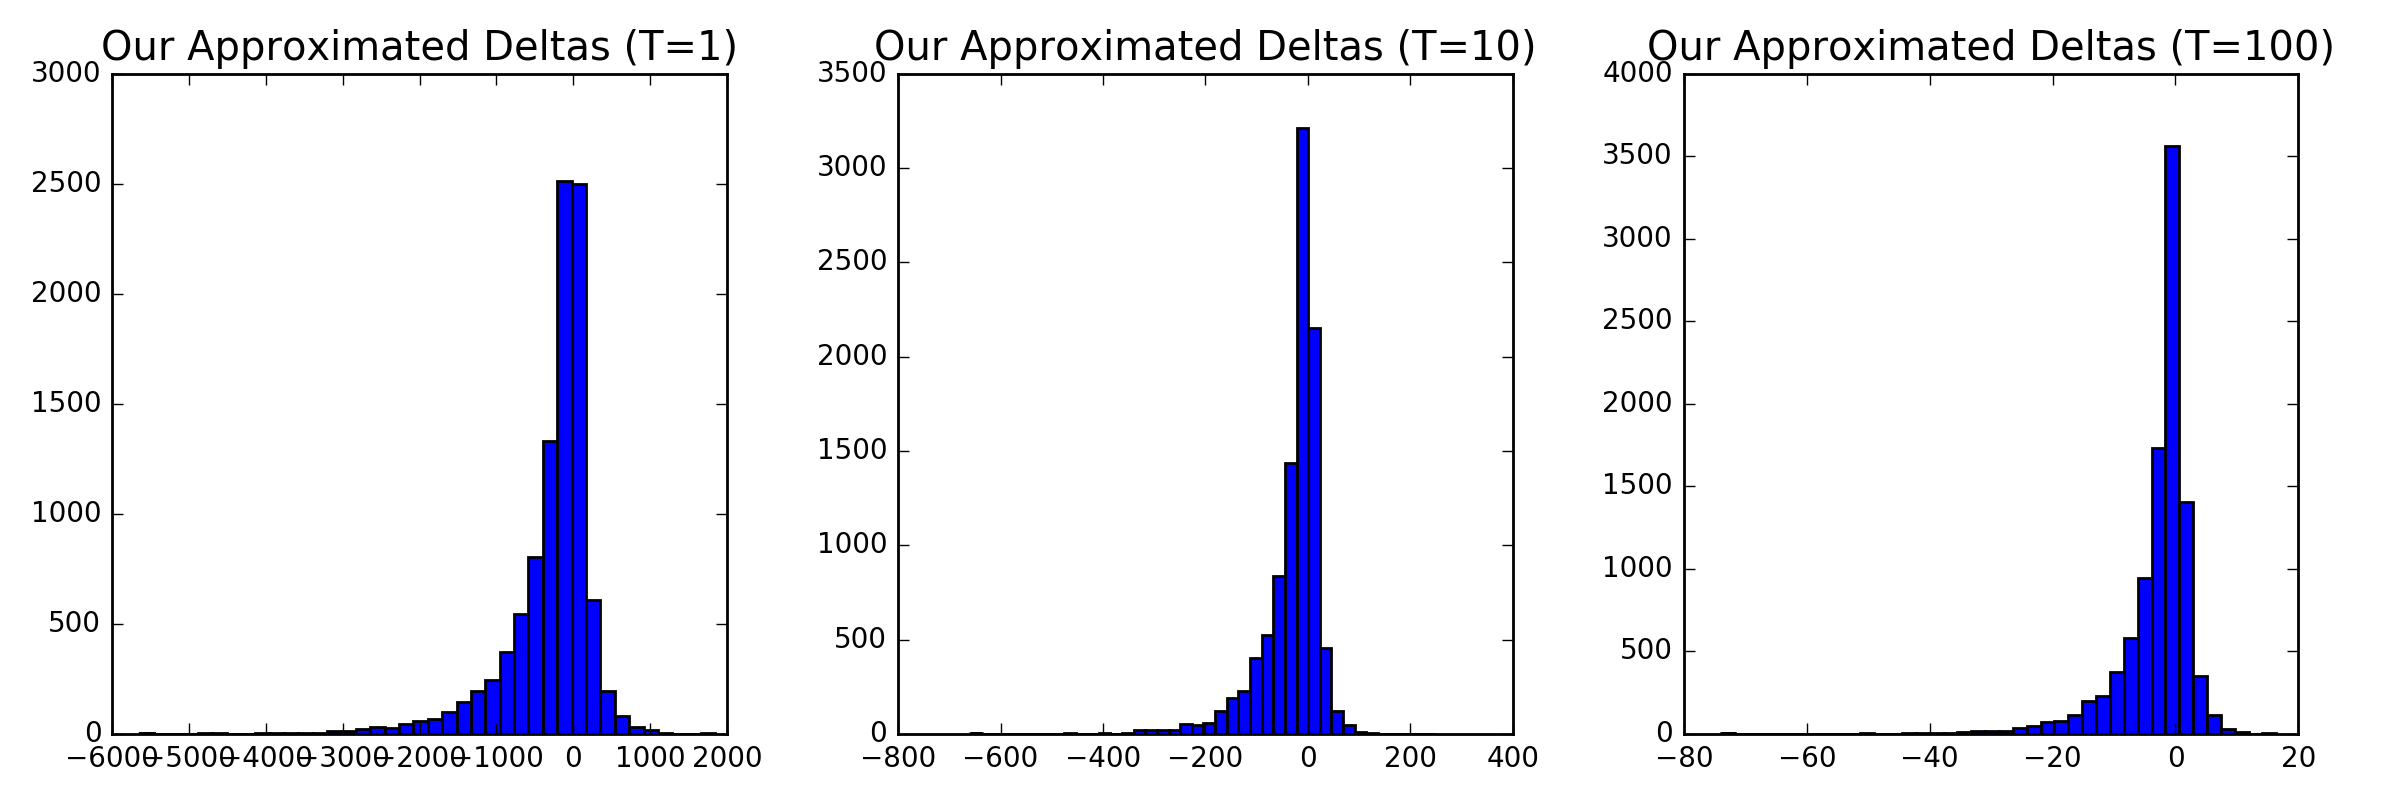
\includegraphics[width=1\linewidth]{our_deltas_v01.png}
  \caption{Our $\Delta'$ values for three different temperature values.}
  \label{fig:diagnostics1}
\end{figure}

\begin{figure}[ht]
  \centering
  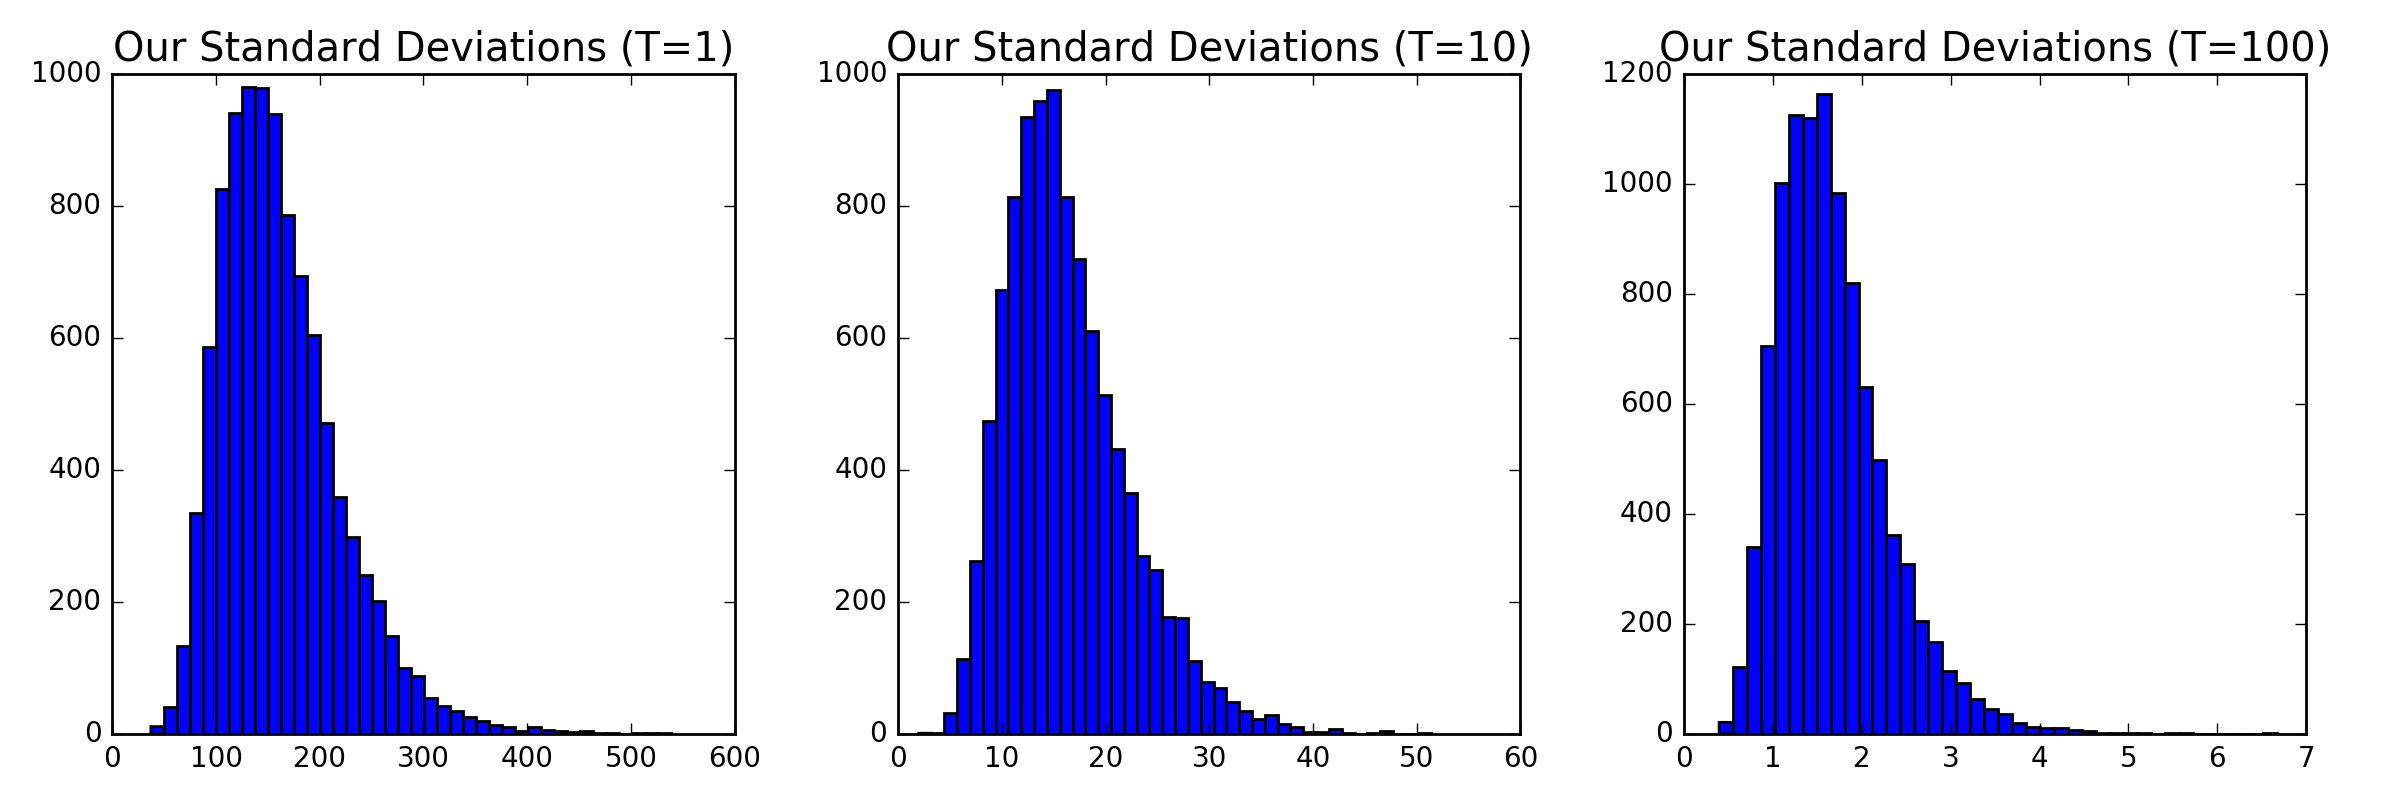
\includegraphics[width=1\linewidth]{our_sds_v01.png}
  \caption{Our ${\rm std}(\Delta')$ values for three different temperature values.}
  \label{fig:diagnostics2}
\end{figure}

\begin{figure}[ht]
  \centering
  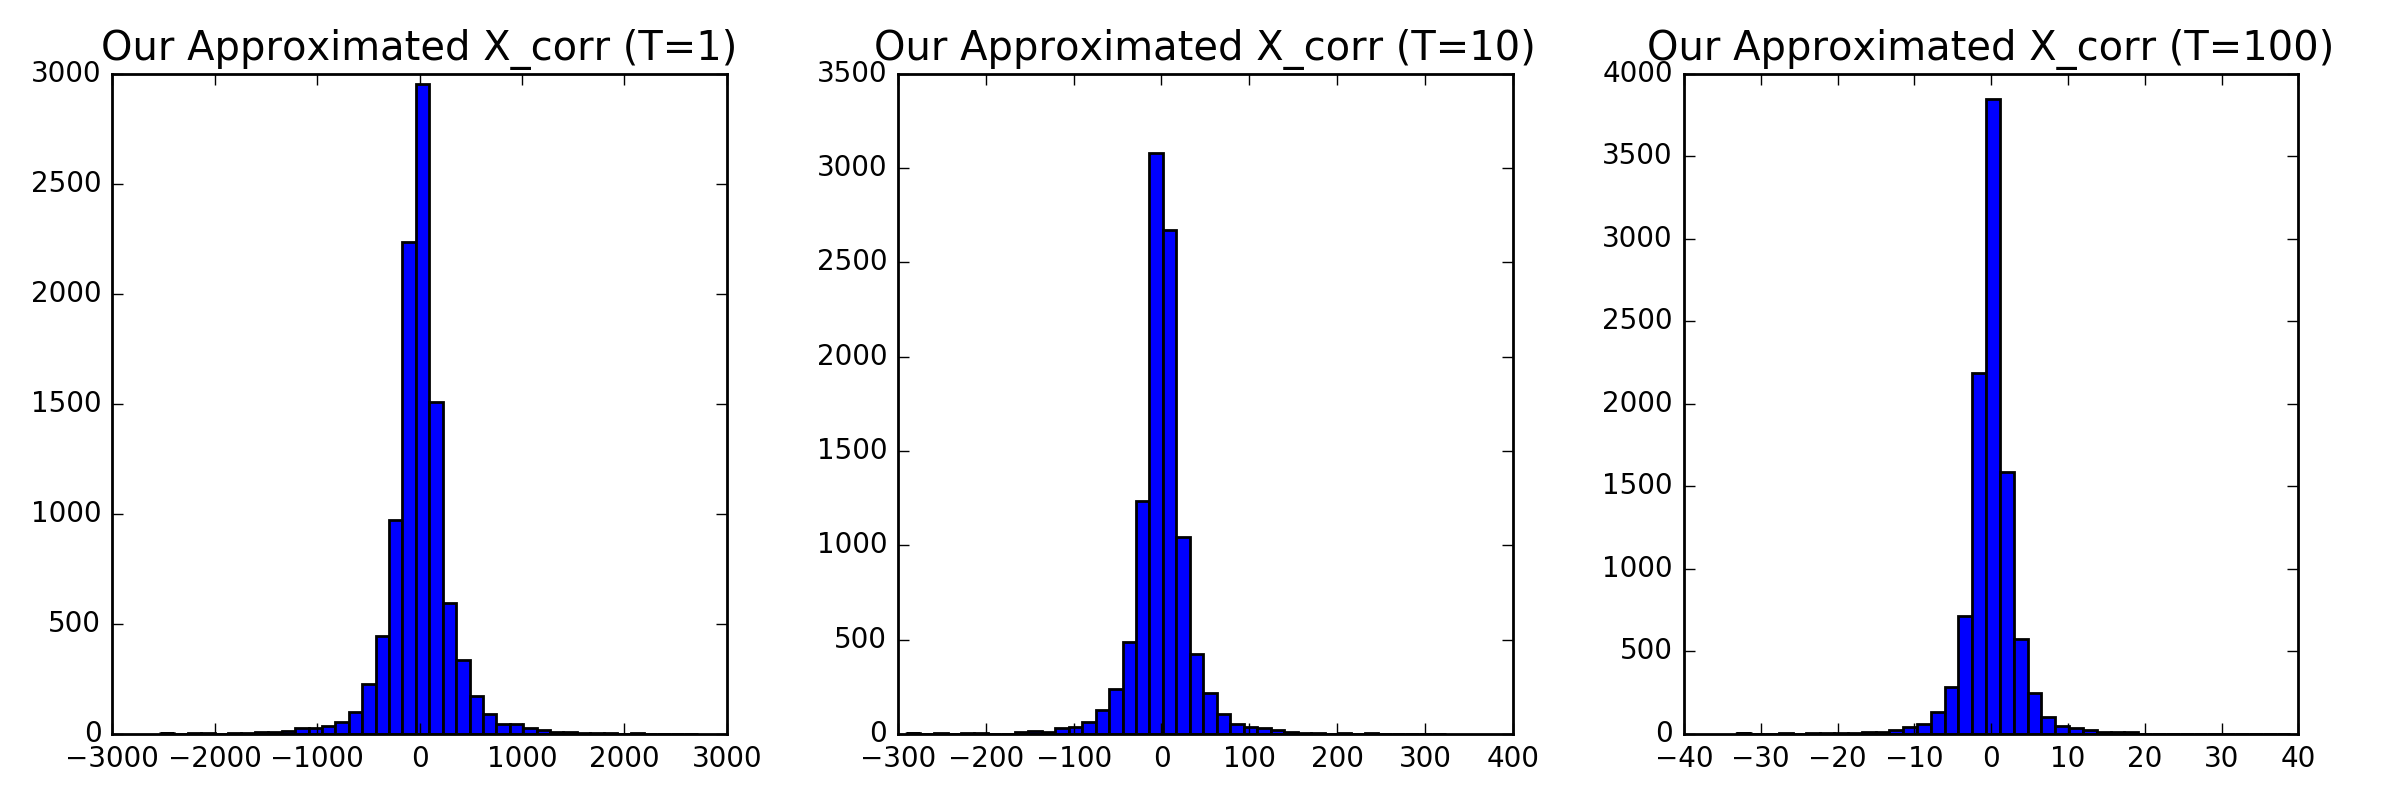
\includegraphics[width=1\linewidth]{our_xcorrs_v01.png}
  \caption{Our $X_{\rm corr}$ values for three different temperature values.}
  \label{fig:diagnostics3}
\end{figure}



\section{Logistic Regression Experiment Details}

{\color{blue}
Daniel: TODO
}

\section{Neural Network Experiment Details}

{\color{blue}
Daniel: TODO
}

% Daniel: here are example LaTeX codes for figures and tables if we want to use them.
%\begin{figure}[h]
%  \centering
%  \fbox{\rule[-.5cm]{0cm}{4cm} \rule[-.5cm]{4cm}{0cm}}
%  \caption{Sample figure caption.}
%\end{figure}
%\begin{table}[t]
%  \caption{Sample table title}
%  \label{sample-table}
%  \centering
%  \begin{tabular}{lll}
%    \toprule
%    \multicolumn{2}{c}{Part}                   \\
%    \cmidrule{1-2}
%    Name     & Description     & Size ($\mu$m) \\
%    \midrule
%    Dendrite & Input terminal  & $\sim$100     \\
%    Axon     & Output terminal & $\sim$10      \\
%    Soma     & Cell body       & up to $10^6$  \\
%    \bottomrule
%  \end{tabular}
%\end{table}
%\usepackage[pdftex]{graphicx} ...
%\includegraphics[width=0.8\linewidth]{myfile.pdf}

\end{document}
